\documentclass[supercite]{HustGraduPaper}
%进行个人信息设置
\title{AI+计算机的可能创新途径的分析} %论文题目
\author{王李超} %作者姓名
\date{\today} %日期,默认当日
\school{计算机科学与技术学院} %院系名称
\classnum{计算机科学与技术专业启明2401} %专业班级
\stunum {U202414887} %学号
\instructor{雷鑑铭} %指导教师姓名

%添加自己要用的其他宏包
\usepackage{xltxtra}
\usepackage{bm}
\usepackage[UTF8,heading = true]{ctex}

\begin{document}
	%生成标题页 
	\maketitle[line length=16em]
	%可选参数:
	% logo color=green/black 华中科技大学字样的颜色,绿色或者黑色,默认绿色
	% line length=16em 填写信息处横线的长度,默认12em
	% line font=huawenzhongsong 填写信息的字体,默认huawenzhongsong
	% \maketitle
	
	%生成声明与授权书页 \statement[可选参数]
	%可选参数:
	%confidentiality=yes/no/true/false/empty 是否保密,yes/true为保密;no/false为不保密,empty为不填,默认为empty
	%year=5 保密年数,默认为空
	% \statement
	
	\clearpage %结束上一页
	\pagenumbering{Roman} %摘要页码为大写罗马数字
	
	%填写中文摘要内容和关键字
	\begin{cnabstract}{人工智能;编程;创新}
		2020年,ChatGPT的问世标志着人工智能发展的重要里程碑,也被后世称为“AI元年”。随着AI技术的快速演进,大模型的应用领域从语言生成扩展到视频生成(如Sora)、编程辅助(如Copilot)和图片生成(如MidJourney)等多个方向。作为计算机科学与技术专业的学生,我深刻体会到AI工具在学习与实践中的重要作用。然而,AI在编程领域的潜力远不止于代码生成和调试。本论文从理论角度出发,探讨AI在编程中的创新应用场景与可能的实现方法,包括代码优化、算法改进及架构设计的智能化支持。本文旨在展望AI技术未来的发展方向,并为推动计算机科学的进步提供参考。
	\end{cnabstract}
	%填写英文摘要内容和关键字
	\begin{enabstract}{AI;programming;innovation}
		The emergence of ChatGPT in 2020 marked a pivotal milestone in the evolution of artificial intelligence, earning it the title "Year of AI." With the rapid advancement of AI technologies, large models have expanded their applications beyond language generation to fields such as video creation (e.g., Sora), programming assistance (e.g., Copilot), and image generation (e.g., MidJourney). As a computer science student, I have witnessed the growing impact of AI tools in both learning and practice. However, the potential of AI in programming extends far beyond code generation and debugging. This paper explores theoretical perspectives on innovative applications of AI in programming, including code optimization, algorithm enhancement, architectural design, and intelligent project management. The study aims to envision future directions for AI development while contributing insights to the progress of computer science.
	\end{enabstract}
	
	%生成目录 \tableofcontents[可选参数]
	%可选参数:
	%pagenum=yes/no/true/false 目录是否显示页码,默认为false
	%toc in toc=yes/no/true/false 目录中是否有目录及其页码,默认为false
	%level=4 目录级数,默认是4,即显示到subsubsubsection
	%section indent=0em 目录第一级的缩进,默认是0em
	%subsection indent=1.5em 目录第二级的缩进,默认是1.5em
	%subsubsection indent=3.8em 目录第三级的缩进,默认是3.8em
	%subsubsubsection indent=7em 目录第四级的缩进,默认是7em
	%paragraph indent=11em 目录第五级的缩进,默认是11em
	%subparagraph indent=13em 目录第六级的缩进,默认13em
	%indent=normal/noindent/hustnoindent/sameforsubandsubsub 快速缩进设置,具体见文档
	%dot sep=4.5 目录点间距,默认4.5
	%section dot sep=4.5 目录第一级的点间距,默认是4.5
	%subsection dot sep=4.5 目录第二级的点间距,默认是4.5
	%subsubsection dot sep=4.5 目录第三级的点间距,默认是4.5
	%subsubsubsection dot sep=4.5 目录第四级的点间距,默认是4.5
	%paragraph dot sep=4.5 目录第五级的点间距,默认是4.5
	%subparagraph dot sep=4.6 目录第六级的点间距,默认是4.5
	%请注意在合适的位置放置\pagenumbering{numstyle}使用新的页码
	\tableofcontents[pagenum=yes]
	
	\clearpage%结束上一页
	\pagenumbering{arabic} %正文页码为阿拉伯数字
	
	%正文内容从这里开始
	\section{代码优化}
		事实上,由于人工智能本身就是编程的结果、代码的呈现,有谚语“解铃还须系铃人”,从这个方面看,AI可能比人类更懂代码也就不足为奇了。以下将从自动化性能优化、智能资源管理、语义级别的代码重构三个方面具体探讨。
	% \par 也可以通过\verb|\par|命令来新起一段
	\subsection{自动化性能优化}
		AI在性能优化方面可以通过深度学习模型和静态分析工具的结合,自动发现代码中存在的性能瓶颈。例如,对于复杂的循环结构,AI可以分析每次迭代的时间复杂度,检测是否存在重复计算、内存浪费等问题,进而建议替代方案,如使用缓存(memoization)减少重复计算,或者用矢量化操作加速矩阵运算。对于计算密集型任务,AI还能够识别适合并行化的部分,通过生成多线程或多进程的实现来提升性能。此外,AI还能动态调整算法参数,例如机器学习模型中的超参数,优化性能与资源使用之间的平衡。在大规模分布式系统中,AI还可根据运行时监控信息,实时分析系统的负载分布,优化任务调度策略,减少因资源争用而导致的性能下降。这种自动化的性能优化不仅可以减轻开发者的工作量,还能大幅提高代码在不同场景下的执行效率。
	\subsection{智能资源管理}
	AI在资源管理方面的优化能力主要体现在内存、CPU、GPU等硬件资源的合理分配上。例如,在内存管理中,AI可以通过静态分析预测可能的内存泄漏或高内存占用点,并建议优化策略,如减少不必要的对象分配、改进数据结构的选择等。动态资源管理中,AI能够基于运行时的内存使用情况调整垃圾回收机制,避免内存碎片化或高延迟问题。在多核CPU或GPU加速场景下,AI可以根据任务特性,将计算任务划分为更细粒度的子任务,并自动分配到适当的核心上执行,提升并行效率。在大数据处理环境中,AI可以动态调整数据分片策略、优化I/O操作,避免瓶颈节点的出现。这种基于硬件特性的资源管理优化,可以帮助开发者最大限度地挖掘硬件性能潜力,尤其适用于高性能计算和云计算场景。
	\subsection{语义级别的代码重构}
	AI通过深度学习模型理解代码的功能语义后,可以自动进行代码重构,使代码不仅在功能实现上正确,还符合最佳实践。例如,AI可以识别出存在耦合的代码模块,推荐将其拆分为独立的函数或类,从而提高代码的可维护性和复用性。对于存在冗余逻辑的部分,AI可以通过模式匹配发现重复代码,并建议抽象为通用函数。与此同时,AI还能识别不符合命名规范的变量或函数名称,并建议更具描述性的命名,以提升代码可读性。在重构过程中,AI还会关注性能优化,如将低效的算法逻辑替换为更优的实现。此外,AI还能根据代码历史或团队的开发风格,自动调整代码格式,使整个代码库风格统一,便于协作和审查。这种语义级别的自动化重构,不仅减轻了开发者手动修改代码的负担,还显著提高了软件的质量与可维护性。
	
	% \verb|\subsubsubsection|是本样式定义的第四级标题,其使用方法与前三级相同。
	
	% \paragraph{段落}\label{para:para}这是一个带有顶头标签的段落这是一个带有顶头标签的段落这是一个带有顶头标签的段落这是一个带有顶头标签的段落这是一个带有顶头标签的段落这是一个带有顶头标签的段落这是一个带有顶头标签的段落
	% \subparagraph{小段落}\label{subpara:subpara}只是一个带有缩进标签的段落只是一个带有缩进标签的段落只是一个带有缩进标签的段落只是一个带有缩进标签的段落只是一个带有缩进标签的段落只是一个带有缩进标签的段落只是一个带有缩进标签的段落
	\section{算法改进}
	\subsection{现有经典算法的启发}
	许多人类设计的经典算法具有深远影响。例如:
	\par {\songti \bfseries 排序算法:}如快速排序(QuickSort),其基于分治思想在实际应用中表现出卓越的时间效率。
	\par {\songti \bfseries 图算法:}如Dijkstra算法,解决了单源最短路径问题,并广泛应用于导航和网络路由。
	\par {\songti \bfseries 搜索算法:}如A*算法,结合了启发式搜索和代价函数,是路径规划领域的核心算法。
	\par {\songti \bfseries 机器学习算法:}如支持向量机(SVM)和随机森林,这些算法在人类精心设计的基础上实现了分类和回归任务的高效解决方案。
	\par 尽管这些算法已经非常成熟,但它们也存在改进空间。例如,Dijkstra算法在稀疏图中效率较低,A*算法的性能依赖于启发函数的质量,而QuickSort在数据接近有序时表现不佳。

	\subsection{AI在改进算法中的角色}
	AI可以通过以下几个途径在算法设计与改进中发挥作用:
	\subsubsection{\songti \bfseries 基于深度学习的启发式优化}
	AI可以通过强化学习或深度学习方法自动生成启发式函数。例如,在A*算法中,AI可以通过大量训练数据,学习到更加精准的启发式估计函数,从而提升路径搜索的效率。类似地,AI可以优化其他启发式算法的评估策略,使其在特定应用场景下表现更加出色。
	\subsubsection{\songti \bfseries 自动化算法结构生成}
	通过神经架构搜索(NAS)技术,AI能够生成优化的算法结构。例如,在排序问题上,AI可以尝试不同的数据划分策略与比较方法,自动生成比QuickSort更高效的排序算法,尤其针对特定的数据分布(如高度有序或高度重复的数据)。这种方法能够跳出传统算法设计的范式,探索新的可能性。
	\subsubsection{\songti \bfseries 混合算法的创新性融合}
	AI可以分析不同算法的特点,生成结合多种优点的新型混合算法。例如,针对图最短路径问题,AI可以结合Dijkstra算法的确定性和A*算法的启发式特点,生成动态调整启发式的混合算法,从而在稀疏图和密集图中都表现良好。
	\subsubsection{\songti \bfseries 针对硬件优化的算法设计}
	AI可以设计更加贴合现代硬件特性的算法。例如,在GPU或TPU环境下,AI可以自动调整算法的并行化粒度,优化线程调度和内存访问模式,从而提升性能。例如,传统的矩阵乘法算法在深度学习中应用广泛,AI可以结合硬件特性优化分块策略,开发出更加高效的计算方案。
	\subsubsection{\songti \bfseries 动态适应性的算法改进}
	传统算法通常是静态的,而AI可以设计具有动态适应性的算法。例如,AI可以开发一种基于遗传算法的动态优化算法,根据实时数据动态调整参数或搜索空间。这样,算法可以在不同的输入场景下自动适配,始终保持高效运行。

	\section{架构设计}
	在重构过程中
	
	% 本模板已经引入伪加粗和伪斜体,这样就不需要对应的粗体和斜体字体也能生成需要的效果,就像下面这样
	
	% {\songti \bfseries 宋体加粗}
	
	% {\songti \itshape 宋体斜体}
	
	% {\songti \bfseries \itshape 宋体粗斜体}
	
	% 请注意,使用加粗和斜体时,请与字体名称一同使用,否则会自动将粗体匹配为黑体,斜体匹配为楷体,就像下面这样
	
	% {正常显示宋体}
	
	% {\bfseries 加粗后变为黑体}
	
	% {\itshape 斜体后变为楷体}
	
	% \section{新的大节}
	% 新的大节会自动出现在新的一页上
	% \section{参考文献和交叉引用}\label{sec:ref}
	% \subsection{参考文献}
	% 这是一个参考文献引用的范例\cite{Stone_1998},你可以随时使用两种不同的样式\normalcite{Stone_1998}或者\supercite{Stone_1998}
	
	% 这样可以添加一个不标注的参考文献引用\nocite{9787508342894}
	
	% 这样可以添加所有bib文件中的参考文献\nocite{*}
	
	% \subsection{交叉引用}\label{subsec:crossref}
	% 本模板已经重写了hyperref宏包的\verb|\autoref|命令,方便引用章节、公式和图表。
	
	% 比如说\autoref{sec:ref}和\autoref{subsec:crossref}就引用了本章节,\autoref{para:para}和\autoref{subpara:subpara}引用了之前的两个段落。显然段落因为没有序号,引用结果和上一节的需要相同,因此建议使用段落“\nameref{para:para}”和段落“\nameref{subpara:subpara}”。
	
	% 本样式定义的第四级标题也可以引用,就像这样:\autoref{subsubsubsec:subsubsubsec}。
	
	
	
	% \section{公式这么用}
	% 在文中引用公式可以这么写:$a^2+b^2=c^2$这是勾股定理,他还可以表示为$c=\sqrt{a^2+b^2}$,还可以让公式单独一段并且加上编号
	% \begin{equation}
	% \sin^2{\theta}+\cos^2{\theta}=1 \label{eq:pingfanghe}
	% \end{equation}
	% 还可以通过添加标签在正文中引用公式,如式~\eqref{eq:pingfanghe}~或者\autoref{eq:pingfanghe}。我们还可以轻松打出一个矩阵
	% \begin{equation}
	% \bm{A}=\begin{bmatrix}
	% 1&2&3&4\\
	% 11&22&33&44\\
	% \end{bmatrix}
	% \times\begin{bmatrix}
	% 22&24\\
	% 32&34\\
	% 42&44\\
	% 52&54\\
	% \end{bmatrix}
	% \end{equation}
	% 或者多个带编号的公式
	% \begin{eqnarray}
	% f_1(x)=12x^2+36x+\sin x\\
	% f_2(x)=\sqrt{3}{x^3+3x}
	% \end{eqnarray}
	% 以上
	
	% \section{用图和表的示例}
	% \subsection{图的使用}
	% \XeLaTeX 环境下可以使用EPS、PDF、PNG、JPEG、BMP格式的图片,当然也可以用绘图包直接在\LaTeX 中绘制图形,推荐使用宏包tikz。图的环境是figure,但figure环境使用复杂且不自带标题,因此本模板定义了一个通用版本的generalfig,该环境会将figure内的图片居中并设置标签与引用名,同时会让图片位置设置为所有可行位置(htbp,即此处、页顶、页底、独立一页),此选项可以作为可选参数设置。
	
	% 其使用方法如下:
	
	% \begin{generalfig}[htb]{大数据信息处理框架}{fig:data}
	% 	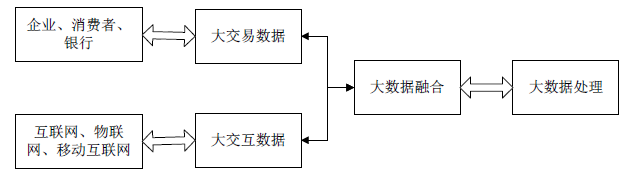
\includegraphics[width=\textwidth]{Figures/data.png}
	% \end{generalfig}
	
	% 同时也可以引用该图片例如:\autoref{fig:data}。请注意generalfig第一个参数是标题,第二个参数是引用。
	
	% \newpage
	
	% \subsection{表的使用}
	% 作为论文,推荐使用三线表进行排版。所谓三线表,即在标题前有横线,标题后有横线,表格最后还有横线,其他地方无线。当然这不是死规定,也可以根据需要在合适的地方加线。
	
	% 本文定义了新的可变长度左中右(LCR)格式,LCR三个格式会根据表格宽度的设定自行控制宽度,且其宽度相等,方便设置和页面相同宽度的表格。但该功能需要使用tabularx做表。
	% \begin{generaltab}{某校学生升高体重样本}{tab:heightweight}
	% 	\begin{tabularx}{\textwidth}{lCCC}
	% 		\toprule
	% 		序号&年龄&身高&体重\\
	% 		\midrule
	% 		1&14&156&42\\
	% 		2&16&158&45\\
	% 		3&14&162&48\\
	% 		4&15&163&50\\
	% 		\cmidrule{2-4} %添加2-4列的中线
	% 		平均&15&159.75&46.25\\
	% 		\bottomrule
	% 	\end{tabularx}
	% \end{generaltab}
	
	% 当然你也可以引用表格,就像这样:\autoref{tab:heightweight}。
	
	% \section{列表的使用}
	% 这是一个计数的列表
	% \begin{enumerate}
	% 	\item 第一项
	% 		\begin{enumerate}
	% 			\item 第一项中的第一项
	% 			\item 第一项中的第二项
	% 		\end{enumerate}
	% 	\item 第二项
	% 	\item 第三项
	% \end{enumerate}

	% 这是一个不计数的列表
	% \begin{itemize}
	% 	\item 第一项
	% 	\begin{itemize}
	% 		\item 第一项中的第一项
	% 		\item 第一项中的第二项
	% 	\end{itemize}
	% 	\item 第二项
	% 	\item 第三项
	% \end{itemize}
	
	\begin{thankpage}
		感谢老师感谢老师感谢老师感谢老师感谢老师感谢老师感谢老师感谢老师感谢老师感谢老师感谢老师感谢老师感谢老师感谢老师感谢老师感谢老师感谢老师感谢老师感谢老师感谢老师感谢老师感谢老师感谢老师感谢老师感谢老师感谢老师感谢老师感谢老师感谢老师感谢老师感谢老师感谢老师感谢老师感谢老师感谢老师感谢老师
		
		感谢老师感谢老师感谢老师感谢老师感谢老师感谢老师感谢老师感谢老师感谢老师感谢老师感谢老师感谢老师感谢老师感谢老师感谢老师感谢老师感谢老师感谢老师感谢老师感谢老师感谢老师感谢老师感谢老师感谢老师感谢老师感谢老师
	\end{thankpage}
	
	%生成参考文献
	%使用方法:\bibliography{参考文件1文件名, 参考文献2文件名, ...}
	% \bibliography{Bibs/mybib}
	
	% \begin{appendices}
	% 	\section{这是第一个附录}
	% 	这里是附录环境,其中的section、subsection、subsubsection已经变为附录的样式,并且会以这种样式加入目录中
	% 	\subsection{附录可以有小节}
	% 	\subsubsection{附录中也可以有小小节}\label{apxsubsubsec:appendix}
	% 	\subsubsubsection{附录中也有小小小节}
	% 	\verb|\autoref|无法识别Appendices环境,引用效果和正文一样,如\autoref{apxsubsubsec:appendix}。所以如果引用附录的话,建议直接使用附录~\ref{apxsubsubsec:appendix}~。
	% \end{appendices}
\end{document}
